% Figura Anexo II: (a) curva de Phillips aumentada y vertical de largo plazo; (b) aceleracionismo: mantener U<Un exige inflación creciente
\documentclass[tikz,border=3pt]{standalone}
\usepackage[T1]{fontenc}
\usepackage[utf8]{inputenc}
\usetikzlibrary{arrows.meta,calc,positioning,decorations.pathreplacing}
\begin{document}
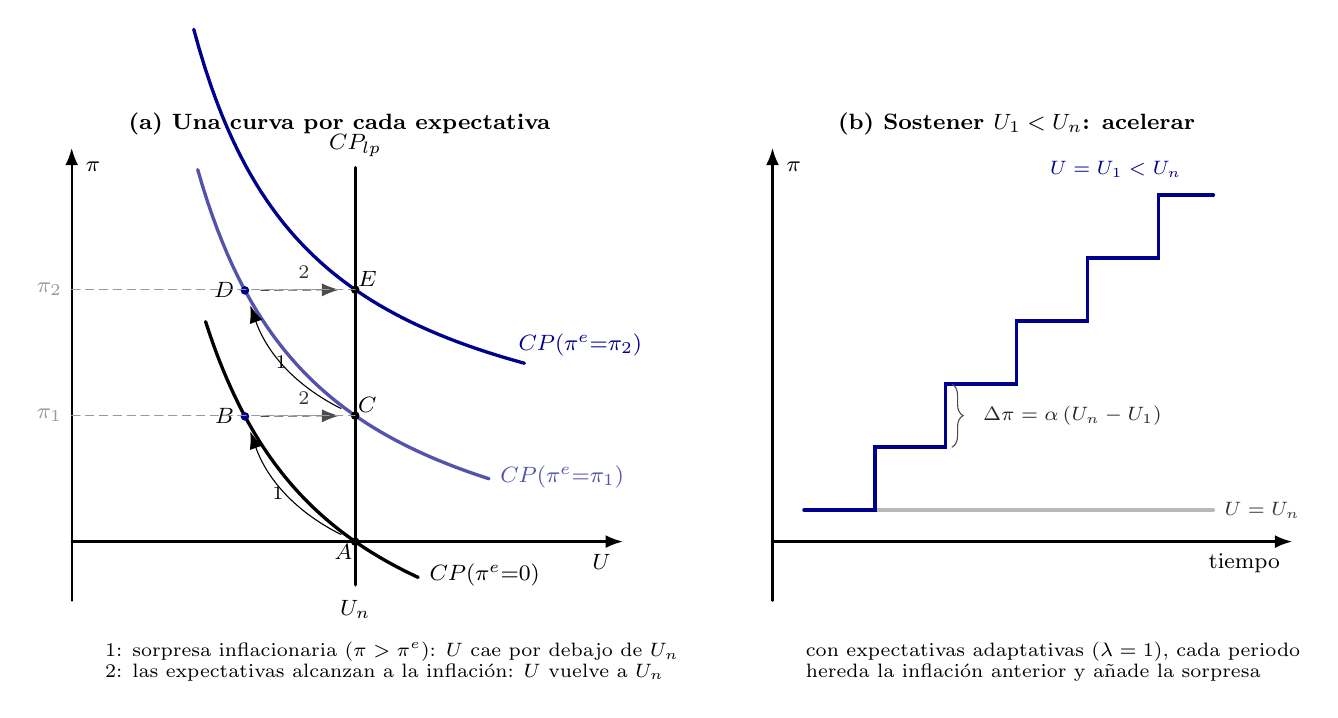
\begin{tikzpicture}[>={Latex[length=2.2mm]}, line cap=round, font=\footnotesize,
  eje/.style={->, thick},
  curva/.style={very thick},
  nueva/.style={very thick, blue!55!black},
  guia/.style={densely dashed, gray!80},
  pto/.style={circle, fill=black, inner sep=1.1pt}]
  % ---------- Panel (a): curvas de corto plazo y vertical de largo plazo ----------
  \node[font=\footnotesize\bfseries] at (3.4,5.3) {(a) Una curva por cada expectativa};
  \draw[eje] (0,-0.75) -- (0,5.0) node[below right=2pt]{$\pi$};
  \draw[eje] (0,0) -- (7.0,0) node[below left=1pt]{$U$};
  % Vertical de largo plazo
  \draw[curva] (3.6,-0.55) -- (3.6,4.75) node[above]{$CP_{lp}$};
  % Curvas de corto plazo: pi = pi^e + 9(1/U - 1/3.6)
  \draw[curva, domain=1.7:4.4, samples=60] plot (\x,{9*(1/\x-0.27778)});
  \node[anchor=west] at (4.42,-0.42) {$CP(\pi^{e}{=}0)$};
  \draw[curva, blue!35!gray, domain=1.6:5.3, samples=60] plot (\x,{1.6+9*(1/\x-0.27778)});
  \node[anchor=west, blue!35!gray] at (5.32,0.82) {$CP(\pi^{e}{=}\pi_1)$};
  \draw[nueva, domain=1.55:5.75, samples=60] plot (\x,{3.2+9*(1/\x-0.27778)});
  \node[anchor=west, blue!55!black] at (5.55,2.5) {$CP(\pi^{e}{=}\pi_2)$};
  % Puntos de la danza
  \node[pto] (A) at (3.6,0) {};
  \node[below left=-2pt of A, inner sep=1pt] {$A$};
  \node[pto, fill=blue!55!black] (B) at (2.2,1.59) {};
  \node[left=1pt of B, inner sep=1pt] {$B$};
  \node[pto] (C) at (3.6,1.6) {};
  \node[above right=-2pt of C, inner sep=1pt] {$C$};
  \node[pto, fill=blue!55!black] (D) at (2.2,3.19) {};
  \node[left=1pt of D, inner sep=1pt] {$D$};
  \node[pto] (E) at (3.6,3.2) {};
  \node[above right=-2pt of E, inner sep=1pt] {$E$};
  \draw[->, shorten >=4pt, shorten <=4pt] (A) to[bend left=22] (B);
  \node at (2.62,0.62) {\scriptsize 1};
  \draw[->, densely dashed, gray!60!black, shorten >=4pt, shorten <=4pt] (B) -- (C);
  \node[gray!40!black] at (2.95,1.82) {\scriptsize 2};
  \draw[->, shorten >=4pt, shorten <=4pt] (C) to[bend left=22] (D);
  \node at (2.66,2.28) {\scriptsize 1};
  \draw[->, densely dashed, gray!60!black, shorten >=4pt, shorten <=4pt] (D) -- (E);
  \node[gray!40!black] at (2.95,3.42) {\scriptsize 2};
  % Guías de inflación
  \draw[guia] (0,1.6) node[left]{$\pi_1$} -- (3.6,1.6);
  \draw[guia] (0,3.2) node[left]{$\pi_2$} -- (3.6,3.2);
  \node[below=2pt] at (3.6,-0.55) {$U_n$};
  \node[align=left, anchor=north west] at (0.3,-1.15) {\scriptsize 1: sorpresa inflacionaria ($\pi>\pi^{e}$): $U$ cae por debajo de $U_n$\\[-2pt]\scriptsize 2: las expectativas alcanzan a la inflación: $U$ vuelve a $U_n$};
  % ---------- Panel (b): aceleracionismo ----------
  \begin{scope}[xshift=8.9cm]
    \node[font=\footnotesize\bfseries] at (3.1,5.3) {(b) Sostener $U_1<U_n$: acelerar};
    \draw[eje] (0,-0.75) -- (0,5.0) node[below right=2pt]{$\pi$};
    \draw[eje] (0,0) -- (6.6,0) node[below left=1pt]{tiempo};
    % En Un: inflación constante
    \draw[curva, gray!55] (0.4,0.4) -- (5.6,0.4) node[right, gray!40!black]{\scriptsize $U=U_n$};
    % En U1 < Un: escalera creciente
    \draw[nueva] (0.4,0.4) -- (1.3,0.4) -- (1.3,1.2) -- (2.2,1.2) -- (2.2,2.0) -- (3.1,2.0) -- (3.1,2.8) -- (4.0,2.8) -- (4.0,3.6) -- (4.9,3.6) -- (4.9,4.4) -- (5.6,4.4);
    \node[anchor=south west, blue!55!black] at (3.4,4.5) {\scriptsize $U=U_1<U_n$};
    \draw[decorate, decoration={brace, amplitude=4pt}, gray!60!black] (2.28,2.0) -- (2.28,1.2);
    \node[anchor=west, gray!30!black] at (2.55,1.6) {\scriptsize $\Delta\pi=\alpha\,(U_n-U_1)$};
    \node[align=left, anchor=north west] at (0.3,-1.15) {\scriptsize con expectativas adaptativas ($\lambda=1$), cada periodo\\[-2pt]\scriptsize hereda la inflación anterior y añade la sorpresa};
  \end{scope}
\end{tikzpicture}
\end{document}
